\documentclass[11pt]{article}

% ============================ PACKAGES ============================
\usepackage[a4paper, margin=2cm]{geometry}
\usepackage[T1]{fontenc}
\usepackage{lmodern}
\usepackage{helvet}                 % Helvetica for headings / labels
\usepackage[table]{xcolor}

% ---------- Colour system (define BEFORE hyperref / tcolorbox) ----------
\definecolor{nsblue}{HTML}{1F6FB2}
\definecolor{nsteal}{HTML}{2BA8A0}
\definecolor{nsgrey}{HTML}{3A3F47}
\definecolor{nslight}{HTML}{EAF3F7}
\definecolor{amber}{HTML}{E0A100}
\definecolor{nsred}{HTML}{C0392B}
\definecolor{nsgreen}{HTML}{2E8B57}
\definecolor{swcol}{HTML}{FDF3E0}

\usepackage{booktabs}
\usepackage{array}
\usepackage{tabularx}
\usepackage{amsmath}
\usepackage{amssymb}
\usepackage{enumitem}
\usepackage{float}
\usepackage{tikz}
\usetikzlibrary{shapes.geometric, arrows.meta, positioning}
\usepackage{tcolorbox}
\tcbuselibrary{breakable}
\usepackage{titlesec}
\usepackage{fancyhdr}
\usepackage[colorlinks=true, linkcolor=nsblue, urlcolor=nsteal, citecolor=nsblue]{hyperref}

% ============================ LAYOUT ============================
\setlength{\parindent}{0pt}
\setlength{\parskip}{0.45em plus 0.1em}
\setlength{\headheight}{14pt}
\setcounter{secnumdepth}{2}
\setcounter{tocdepth}{1}

\newcolumntype{Y}{>{\raggedright\arraybackslash}X}
\newcolumntype{L}{>{\raggedright\arraybackslash}p{2.0cm}}

% ---------- Coloured section headings ----------
\titleformat{\section}
  {\sffamily\Large\bfseries\color{nsblue}}
  {\thesection}{0.6em}{}
  [{\color{nsblue!25}\titlerule[1.2pt]}]
\titlespacing*{\section}{0pt}{1.3em}{0.6em}
\titleformat{\subsection}
  {\sffamily\large\bfseries\color{nsgrey}}
  {\thesubsection}{0.5em}{}
\titlespacing*{\subsection}{0pt}{0.9em}{0.35em}

% ---------- Page header / footer ----------
\pagestyle{fancy}
\fancyhf{}
\fancyhead[L]{\small\sffamily\color{nsgrey}NeuroShield --- 10-Day Build Sprint}
\fancyhead[R]{\small\sffamily\color{nsgrey}\thepage}
\renewcommand{\headrule}{\vskip1pt{\color{nsblue!45}\hrule height 0.8pt}}
\renewcommand{\footrulewidth}{0pt}

% ============================ COMPONENTS ============================
% Inline coloured tag (square, bulletproof: uses xcolor \colorbox only)
\newcommand{\pill}[2]{\colorbox{#1}{\color{white}\footnotesize\sffamily\bfseries #2}}

% One labelled row inside a day card
\newcommand{\trk}[3]{\pill{#1}{#2}\hspace{5pt}#3\par}
\newcommand{\cardrule}{\par\vspace{3pt}{\color{black!12}\rule{\linewidth}{0.6pt}}\par\vspace{4pt}}

% KPI mini-card (minipage + simple tcolorbox)
\newcommand{\kpi}[3]{%
  \begin{minipage}[t]{0.188\linewidth}
  \begin{tcolorbox}[colback=#3!12, colframe=#3, boxrule=1pt, arc=3pt, halign=center,
    left=1pt, right=1pt, top=4pt, bottom=4pt]
  {\large\sffamily\bfseries\color{#3}#1}\\{\scriptsize\sffamily\color{nsgrey}#2}
  \end{tcolorbox}
  \end{minipage}}

% Day card (optional colour arg for milestone days) -- standard skin only
\newtcolorbox{daycard}[2][nsblue]{%
  breakable, colback=white, colframe=#1, boxrule=1pt, arc=3pt,
  left=10pt, right=10pt, top=8pt, bottom=8pt,
  colbacktitle=#1, coltitle=white, fonttitle=\sffamily\bfseries, title={#2}}

% Callout box -- standard skin only
\newtcolorbox{callout}[2][amber]{%
  breakable, colback=#1!8, colframe=#1, boxrule=1pt, arc=2pt,
  left=9pt, right=9pt, top=6pt, bottom=6pt,
  colbacktitle=#1!8, coltitle=#1!75!black, fonttitle=\sffamily\bfseries, title={#2}}

% Table header cell
\newcommand{\hd}[1]{\textbf{\sffamily\textcolor{white}{#1}}}

\begin{document}
\thispagestyle{empty}

% ============================ COVER ============================
\begin{tcolorbox}[colback=nsblue, colframe=nsblue, arc=5pt, boxrule=0pt,
  left=16pt, right=16pt, top=14pt, bottom=14pt]
{\sffamily\color{white}\fontsize{30}{34}\selectfont\bfseries NeuroShield}\\[3pt]
{\sffamily\color{white}\LARGE 10-Day Build Sprint}\\[8pt]
{\sffamily\color{nslight}\normalsize A hands-on plan to build the prototype end-to-end ---
hardware, firmware, data, models, and app.}
\end{tcolorbox}

\vspace{4pt}
{\sffamily\small\color{nsgrey}\textbf{Manika Jhaveri} --- mentored build plan
\hfill Sprint window: 10 working days}

\vspace{10pt}
% ---- KPI row ----
\noindent
\kpi{10}{days}{nsblue}\hfill
\kpi{4}{sensors}{nsteal}\hfill
\kpi{5}{ML models}{amber}\hfill
\kpi{6}{datasets}{nsgreen}\hfill
\kpi{\$20--30}{per month}{nsgrey}

\vspace{10pt}
\begin{callout}[nsblue]{Overview}
This is the practical build companion to the NeuroShield research plan, written to be read
\emph{with the student}. It defines what we build in ten days, the workflow, the system architecture,
a day-by-day sprint with two parallel tracks (hardware/firmware and data/ML), the datasets mapped to
each model, the exact features, the tools we need, and a risk register. The realistic ten-day goal is
a \textbf{working, laptop-connected sensing glove that produces a personalized, explainable
Green/Amber/Red stress readout}; the wireless, on-device version is out of scope for this sprint.
\end{callout}

\vspace{2pt}
{\color{nsblue!30}\hrule height 1pt}
\tableofcontents
{\color{nsblue!30}\hrule height 1pt}

% ============================ 1. OBJECTIVE ============================
\section{Objective and Scope}\label{sec:scope}

One headline deliverable, clear boundaries. Read these four cards first.

\noindent
\begin{minipage}[t]{0.485\linewidth}
\begin{tcolorbox}[title={Goal (by Day 10)}, colframe=nsblue, colbacktitle=nsblue,
  colback=nsblue!5, coltitle=white, fonttitle=\sffamily\bfseries, arc=3pt, boxrule=1pt]
A glove that (1)~reads pulse, skin conductance, temperature, and motion from the hand;
(2)~streams to a laptop; (3)~runs a trained, \emph{personalized} classifier; and (4)~shows a
Green/Amber/Red status \emph{with a plain-language reason}, ignoring readings while the hand moves.
\end{tcolorbox}
\end{minipage}\hfill
\begin{minipage}[t]{0.485\linewidth}
\begin{tcolorbox}[title={In scope}, colframe=nsgreen, colbacktitle=nsgreen,
  colback=nsgreen!5, coltitle=white, fonttitle=\sffamily\bfseries, arc=3pt, boxrule=1pt]
Breadboard sensing $\rightarrow$ streaming $\rightarrow$ feature pipeline $\rightarrow$ per-user
baseline $\rightarrow$ models M1--M3 $\rightarrow$ dashboard with explanation $\rightarrow$ glove
assembly $\rightarrow$ a small local validation (E1, E2).
\end{tcolorbox}
\end{minipage}

\vspace{8pt}
\noindent
\begin{minipage}[t]{0.485\linewidth}
\begin{tcolorbox}[title={Out of scope (later cycle)}, colframe=nsgrey, colbacktitle=nsgrey,
  colback=nsgrey!5, coltitle=white, fonttitle=\sffamily\bfseries, arc=3pt, boxrule=1pt]
The wireless low-power board (XIAO nRF52840, \emph{not yet ordered}); on-device TinyML inference;
a flexible PCB; a phone app; domain adaptation (E3).
\end{tcolorbox}
\end{minipage}\hfill
\begin{minipage}[t]{0.485\linewidth}
\begin{tcolorbox}[title={Parts status}, colframe=amber, colbacktitle=amber,
  colback=amber!8, coltitle=white, fonttitle=\sffamily\bfseries, arc=3pt, boxrule=1pt]
The ordered list already covers the full breadboard build and a first glove. The \textbf{only} future
purchase for the wireless version is the XIAO nRF52840 ($\sim$\$16).
\end{tcolorbox}
\end{minipage}

% ============================ 2. WORKFLOW ============================
\section{Development Workflow}\label{sec:workflow}

Two parallel tracks progress at once and meet only at integration points.

\noindent
\begin{minipage}[t]{0.485\linewidth}
\begin{tcolorbox}[title={Hardware / Firmware}, colframe=nsteal, colbacktitle=nsteal!15,
  coltitle=nsgrey, colback=white, fonttitle=\sffamily\bfseries, arc=3pt, boxrule=1pt]
\pill{nsteal}{HW}\hspace{5pt}Wire sensors, write ESP32-S3 firmware, stream data, assemble the glove.
\end{tcolorbox}
\end{minipage}\hfill
\begin{minipage}[t]{0.485\linewidth}
\begin{tcolorbox}[title={Data / ML}, colframe=amber, colbacktitle=amber!16,
  coltitle=nsgrey, colback=white, fonttitle=\sffamily\bfseries, arc=3pt, boxrule=1pt]
\pill{amber}{SW/ML}\hspace{5pt}Download datasets, build the feature pipeline, train and validate the
models, build the dashboard.
\end{tcolorbox}
\end{minipage}

\subsection{Operating rules}
\begin{enumerate}[leftmargin=1.6em, itemsep=4pt]
\item \textbf{Streaming-first.} The device only \emph{reads and sends}; the laptop does all the
thinking this sprint. This removes the hardest integration risk (on-device inference is deferred).
\item \textbf{One contract between the tracks:} a fixed row format
(\texttt{timestamp, hr, eda, temp, accel\_x/y/z}) at a fixed sample rate. Once it exists (Day~3), the
ML track can work off \emph{recorded} data without the hardware present.
\item \textbf{Version control:} one GitHub repo --- \texttt{firmware/}, \texttt{ml/}, \texttt{app/}
--- committed daily.
\item \textbf{Daily 15-minute check-in:} what shipped, what is blocked, what ships next.
\item \textbf{Test each sensor alone before combining.} Never debug ten things at once.
\end{enumerate}

% ============================ 3. ARCHITECTURE ============================
\section{System Architecture}\label{sec:arch}

\subsection{Wearable and software (development configuration)}

\begin{figure}[H]
\centering
\begin{tcolorbox}[colback=nslight!45, colframe=nsblue!30, boxrule=0.8pt, arc=3pt,
  left=6pt, right=6pt, top=8pt, bottom=8pt, width=\linewidth]
\centering
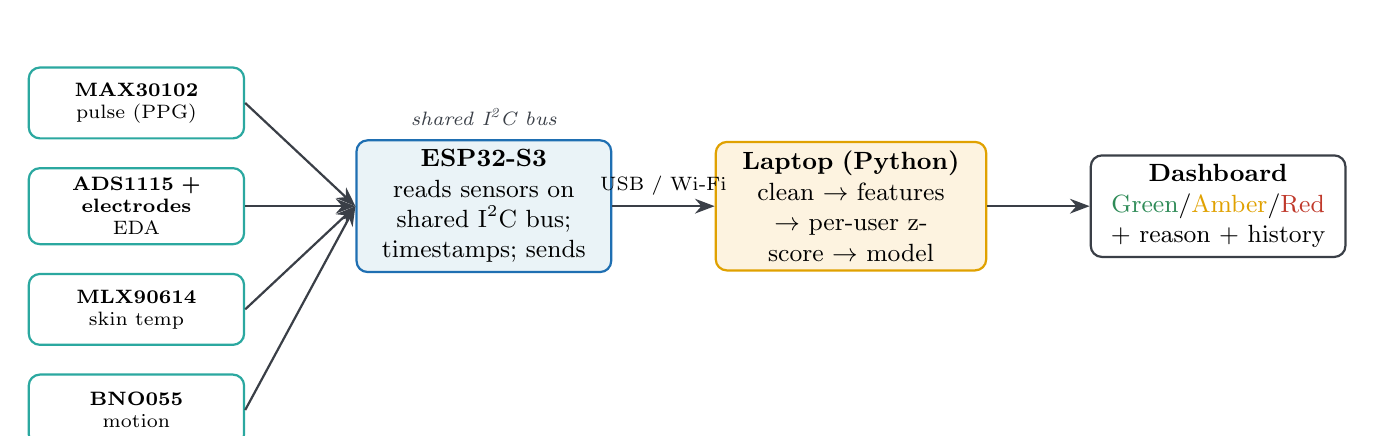
\begin{tikzpicture}[
  node distance=0.9cm and 0.5cm,
  sensor/.style={rectangle, rounded corners, draw=nsteal, fill=white, thick,
    text width=2.5cm, align=center, minimum height=0.9cm, font=\scriptsize},
  brain/.style={rectangle, rounded corners, draw=nsblue, fill=nslight, thick,
    text width=3.0cm, align=center, minimum height=1.1cm, font=\small},
  laptop/.style={rectangle, rounded corners, draw=amber, fill=swcol, thick,
    text width=3.2cm, align=center, minimum height=1.1cm, font=\small},
  outputbox/.style={rectangle, rounded corners, draw=nsgrey, fill=white, thick,
    text width=3.0cm, align=center, minimum height=1.1cm, font=\small},
  arrow/.style={-{Stealth[length=2.5mm]}, thick, draw=nsgrey}
]
\node[sensor] (ppg) {\textbf{MAX30102}\\pulse (PPG)};
\node[sensor, below=0.35cm of ppg] (eda) {\textbf{ADS1115 + electrodes}\\EDA};
\node[sensor, below=0.35cm of eda] (temp) {\textbf{MLX90614}\\skin temp};
\node[sensor, below=0.35cm of temp] (imu) {\textbf{BNO055}\\motion};
\node[brain, right=1.4cm of eda] (mcu) {\textbf{ESP32-S3}\\reads sensors on shared I\textsuperscript{2}C bus; timestamps; sends};
\node[laptop, right=1.3cm of mcu] (lap) {\textbf{Laptop (Python)}\\clean $\to$ features $\to$ per-user z-score $\to$ model};
\node[outputbox, right=1.3cm of lap] (ui) {\textbf{Dashboard}\\\textcolor{nsgreen}{Green}/\textcolor{amber}{Amber}/\textcolor{nsred}{Red} + reason + history};
\draw[arrow] (ppg.east) -- (mcu.west);
\draw[arrow] (eda.east) -- (mcu.west);
\draw[arrow] (temp.east) -- (mcu.west);
\draw[arrow] (imu.east) -- (mcu.west);
\node[font=\scriptsize\itshape, text=nsgrey, above=0.05cm of mcu] {shared I\textsuperscript{2}C bus};
\draw[arrow] (mcu) -- node[above, font=\scriptsize]{USB / Wi-Fi} (lap);
\draw[arrow] (lap) -- (ui);
\end{tikzpicture}
\end{tcolorbox}
\caption{Development architecture. The glove only senses and streams; the laptop does all processing
and inference. The wireless version replaces the laptop link with a XIAO nRF52840 running the model
over BLE (later cycle).}
\end{figure}

\subsection{Data / ML workflow}

\begin{figure}[H]
\centering
\begin{tcolorbox}[colback=nslight!45, colframe=nsblue!30, boxrule=0.8pt, arc=3pt,
  left=6pt, right=6pt, top=8pt, bottom=8pt, width=\linewidth]
\centering
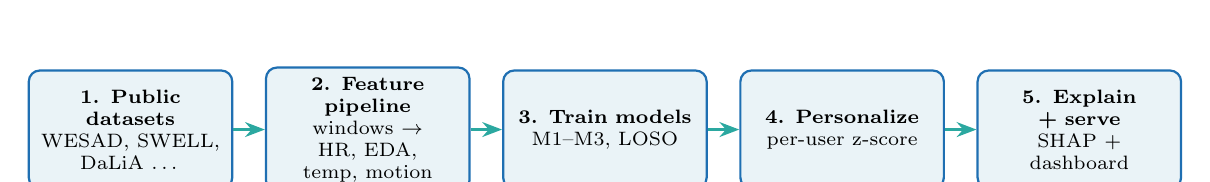
\begin{tikzpicture}[
  node distance=0.4cm,
  stage/.style={rectangle, rounded corners, draw=nsblue, fill=nslight, thick,
    text width=2.35cm, align=center, minimum height=1.5cm, font=\scriptsize},
  arrow/.style={-{Stealth[length=2.5mm]}, very thick, draw=nsteal}
]
\node[stage] (s1) {\textbf{1. Public datasets}\\WESAD, SWELL, DaLiA \dots};
\node[stage, right=of s1] (s2) {\textbf{2. Feature pipeline}\\windows $\to$ HR, EDA, temp, motion};
\node[stage, right=of s2] (s3) {\textbf{3. Train models}\\M1--M3, LOSO};
\node[stage, right=of s3] (s4) {\textbf{4. Personalize}\\per-user z-score};
\node[stage, right=of s4] (s5) {\textbf{5. Explain + serve}\\SHAP + dashboard};
\draw[arrow] (s1)--(s2); \draw[arrow] (s2)--(s3); \draw[arrow] (s3)--(s4); \draw[arrow] (s4)--(s5);
\end{tikzpicture}
\end{tcolorbox}
\caption{The same feature pipeline runs on public data (to train) and on the live glove stream (to
predict). Building it once, correctly, is the core of the ML track.}
\end{figure}

% ============================ 4. SPRINT ============================
\section{The 10-Day Sprint}\label{sec:sprint}

Every day is a card with three rows: the \pill{nsteal}{HW} hardware task, the \pill{amber}{SW/ML}
data/ML task, and a \pill{nsgreen}{DONE} acceptance test. Milestone days
(\textcolor{amber}{\textbf{amber}}) are integration checkpoints.

% ---- Timeline hero ----
\begin{figure}[H]
\centering
\begin{tcolorbox}[colback=white, colframe=nsblue!25, boxrule=0.8pt, arc=3pt,
  left=6pt, right=6pt, top=10pt, bottom=6pt, width=\linewidth]
\centering
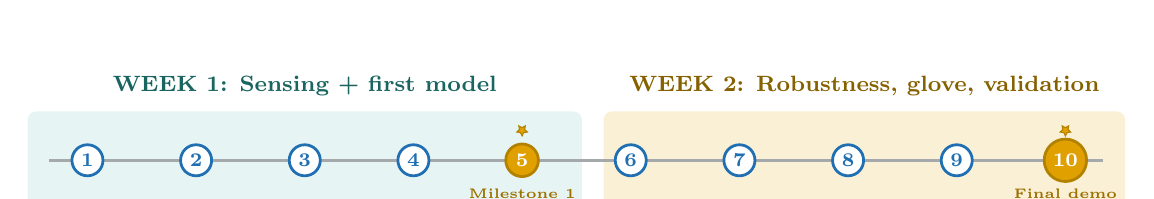
\begin{tikzpicture}[x=1.38cm, font=\sffamily]
\fill[nsteal!12, rounded corners=3pt] (0.45,-0.62) rectangle (5.55,0.62);
\fill[amber!16, rounded corners=3pt] (5.75,-0.62) rectangle (10.55,0.62);
\node[text=nsteal!60!black, font=\footnotesize\bfseries] at (3.0,0.95)
  {WEEK 1: Sensing + first model};
\node[text=amber!60!black, font=\footnotesize\bfseries] at (8.15,0.95)
  {WEEK 2: Robustness, glove, validation};
\draw[nsgrey!45, line width=1.2pt] (0.65,0) -- (10.35,0);
\foreach \d in {1,2,3,4,6,7,8,9}{
  \node[circle, draw=nsblue, fill=white, line width=1pt, inner sep=1.7pt,
    font=\scriptsize\bfseries, text=nsblue] at (\d,0) {\d};
}
\foreach \d in {5,10}{
  \node[circle, draw=amber!80!black, fill=amber, line width=1pt, inner sep=1.9pt,
    font=\scriptsize\bfseries, text=white] at (\d,0) {\d};
  \node[star, star points=5, star point ratio=0.5, draw=amber!80!black, fill=amber,
    inner sep=1.4pt] at (\d,0.38) {};
}
\node[font=\tiny\bfseries, text=amber!70!black] at (5,-0.42) {Milestone 1};
\node[font=\tiny\bfseries, text=amber!70!black] at (10,-0.42) {Final demo};
\end{tikzpicture}
\end{tcolorbox}
\caption{The sprint at a glance: two weeks, ten days, two milestones (Days 5 and 10).}
\end{figure}

\begin{daycard}{DAY 1 --- Setup and foundations}
\trk{nsteal}{HW}{Install Arduino IDE / PlatformIO, add ESP32-S3 board support, blink an LED, confirm
the board is recognized; lay out the breadboard.}
\smallskip
\trk{amber}{SW/ML}{Create the GitHub repo (\texttt{firmware/ ml/ app/}); set up Python with
\texttt{numpy, pandas, scikit-learn, neurokit2, matplotlib, streamlit}; open a Colab notebook; create
Kaggle + PhysioNet accounts; start downloading all six datasets.}
\cardrule
\trk{nsgreen}{DONE}{ESP32-S3 blinks; repo exists; WESAD is downloaded and opens in a notebook.}
\end{daycard}

\begin{daycard}{DAY 2 --- Sensor bring-up (one at a time)}
\trk{nsteal}{HW}{Wire and read \emph{each} sensor individually over I\textsuperscript{2}C: MAX30102
(raw pulse), ADS1115 + finger electrodes (raw EDA voltage), MLX90614 (temperature). Note each
I\textsuperscript{2}C address.}
\smallskip
\trk{amber}{SW/ML}{Load WESAD; isolate the wrist (Empatica~E4) channels (BVP, EDA, TEMP, ACC);
understand the labels (baseline / stress / amusement).}
\cardrule
\trk{nsgreen}{DONE}{Each sensor prints sensible live numbers; WESAD E4 channels are plotted for one
subject.}
\end{daycard}

\begin{daycard}{DAY 3 --- Full integration + the streaming contract}
\trk{nsteal}{HW}{Put all four sensors on the shared I\textsuperscript{2}C bus (add BNO055). Write
firmware that samples at a fixed rate, timestamps, and streams rows over USB serial; write the
laptop-side logger that saves to CSV.}
\smallskip
\trk{amber}{SW/ML}{Build the \textbf{feature-extraction function} (Section~\ref{sec:features}) and run
it on WESAD windows. This is the single most reused piece of code.}
\cardrule
\trk{nsgreen}{DONE}{A CSV of live multi-sensor data is recorded; the feature function turns a window
into a feature row.}
\end{daycard}

\begin{daycard}{DAY 4 --- Baseline calibration + first training}
\trk{nsteal}{HW}{Implement the 2-minute \textbf{calibration routine}: record the wearer at rest,
compute per-feature mean and standard deviation, save them.}
\smallskip
\trk{amber}{SW/ML}{Train \textbf{Model M1} (rest vs.\ stress) on WESAD E4 channels using
leave-one-subject-out (LOSO); report balanced accuracy and macro-F1.}
\cardrule
\trk{nsgreen}{DONE}{A baseline file is produced from a live rest recording; M1 reports a LOSO score.}
\end{daycard}

\begin{daycard}[amber]{DAY 5 --- MILESTONE 1: Live end-to-end demo}
\trk{nsteal}{HW}{Confirm stable, dropout-free streaming for 10+ minutes.}
\smallskip
\trk{amber}{SW/ML}{Wire it together: live stream $\to$ features $\to$ per-user z-score $\to$ M1
$\to$ Green/Amber/Red, printed live. Add SHAP so each prediction lists the top contributing signals.}
\cardrule
\trk{nsgreen}{DONE}{\textbf{You can put the sensors on and the laptop prints a live status and the
reason for it.} Demo recorded.}
\end{daycard}

\begin{daycard}{DAY 6 --- Motion robustness (M3) + cognitive load (M2)}
\trk{nsgrey}{HW}{\textit{No hardware task --- the glove already streams.}}
\smallskip
\trk{amber}{SW/ML}{\textbf{M3:} use BNO055 acceleration magnitude to detect motion and \emph{suppress}
inference in high-motion windows; sanity-check against PPG-DaLiA. \textbf{M2:} train a cognitive-load
classifier on SWELL-KW (HRV + EDA).}
\cardrule
\trk{nsgreen}{DONE}{Status shows ``motion --- paused'' when the hand moves; M2 has a LOSO score.}
\end{daycard}

\begin{daycard}{DAY 7 --- Local validation experiments (E1, E2)}
\trk{nsteal}{HW}{Run the acute-stress protocol on 2--3 volunteers wearing the device: rest $\to$
Stroop task $\to$ timed mental arithmetic $\to$ recovery, labelling each phase.}
\smallskip
\trk{amber}{SW/ML}{\textbf{E1:} test M1 (trained on WESAD) on this locally collected data --- how much
accuracy survives cheap hardware? \textbf{E2:} compare M1 with vs.\ without per-user z-scores.}
\cardrule
\trk{nsgreen}{DONE}{A small labelled local dataset exists; E1 and E2 produce numbers and confusion
matrices.}
\end{daycard}

\begin{daycard}{DAY 8 --- Glove assembly}
\trk{nsteal}{HW}{Move off the breadboard: MAX30102 on a fingertip, two Ag/AgCl electrodes on adjacent
finger pads, electronics (ESP32-S3, BNO055, ADS1115) on the back of the hand on perfboard. Solder,
insulate with heat-shrink, secure with medical tape and velcro, attach the LiPo + TP4056; re-run the
sensor check.}
\smallskip
\trk{nsgrey}{SW/ML}{\textit{No software task --- the pipeline is unchanged.}}
\cardrule
\trk{nsgreen}{DONE}{The glove streams the same data the breadboard did, now on the hand.}
\end{daycard}

\begin{daycard}{DAY 9 --- Dashboard + offline models (M4, M5)}
\trk{nsgrey}{HW}{\textit{No hardware task --- software focus.}}
\smallskip
\trk{amber}{SW/ML}{Build the \textbf{Streamlit dashboard}: live Green/Amber/Red, the ranked ``why''
panel, and a simple history view. Add \textbf{M4} (thermal-strain trend from temp+HR, WESAD) and
\textbf{M5} (longitudinal recovery trend, Fitbit dataset) as \emph{offline} analyses/plots.}
\cardrule
\trk{nsgreen}{DONE}{The dashboard shows live status + reason + history; M4/M5 plots exist in the repo.}
\end{daycard}

\begin{daycard}[amber]{DAY 10 --- MILESTONE 2: Full demo, results, write-up}
\trk{nsteal}{HW}{Full end-to-end test on the glove; freeze results (E1/E2 tables, confusion
matrices); record the final demo.}
\smallskip
\trk{amber}{SW/ML}{Write a 2-page results memo; update the repo README; note next-cycle work (order
the nRF52840, port the model to TFLite Micro / Edge Impulse).}
\cardrule
\trk{nsgreen}{DONE}{Glove $\to$ dashboard works front-to-back; results and demo are captured; the repo
is clean.}
\end{daycard}

\begin{callout}[nsred]{If time runs short --- protect this order, cut from the bottom}
\begin{enumerate}[leftmargin=1.5em, itemsep=2pt, nosep]
\item Live sensing + M1 demo (Day~5) --- \textbf{non-negotiable}.
\item Glove assembly (Day~8).
\item E1/E2 numbers (Day~7).
\end{enumerate}
\vspace{2pt}
\textbf{Cut first:} M2, M4, M5, and dashboard polish.
\end{callout}

% ============================ 5. DATASETS ============================
\section{Datasets and Models}\label{sec:data}

All six datasets are free (academic / Kaggle / PhysioNet). Personalization (per-user z-score) applies
to M1 and M2.

{\rowcolors{2}{nslight}{white}
\begin{tabularx}{\linewidth}{@{}L c Y@{}}
\rowcolor{nsblue} \hd{Dataset} & \hd{Model} & \hd{Role and channels used} \\
WESAD (15) & M1, M4 & Primary training for rest-vs-stress; supplies temp+HR to M4. E4: BVP, EDA, TEMP, ACC. \\
Stress-Predict (35) & M1 & Independent validation of M1. E4: BVP, IBI, HR. \\
Nurse Stress (15) & M1 & Naturalistic validation (hospital shifts); motivates personalization. E4: EDA, BVP, HR, TEMP, ACC. \\
PPG-DaLiA (15) & M3 & Train/validate motion-artifact rejection and HR-under-motion (ECG ground truth). PPG, ACC, ECG. \\
SWELL-KW (25) & M2 & Primary training for cognitive-load classification. HRV, EDA. \\
Consumer activity (30) & M5 & Longitudinal recovery-trend demonstration (offline). HR, activity, sleep. \\
\end{tabularx}}

\vspace{6pt}
{\rowcolors{2}{nslight}{white}
\begin{tabularx}{\linewidth}{@{}c Y L@{}}
\rowcolor{nsteal} \hd{Model} & \hd{Task and algorithm} & \hd{Metric} \\
M1 & Rest vs.\ stress (headline); random forest / logistic regression & Bal.\ acc., macro-F1 (LOSO) \\
M2 & Cognitive-load classification; random forest & Bal.\ acc., macro-F1 (LOSO) \\
M3 & Motion detection / HR gating; threshold on accel + HR recovery & HR error (bpm) vs.\ ECG \\
M4 & Thermal-strain trend (offline); trend on temp+HR & Qualitative trend \\
M5 & Longitudinal recovery (offline); trend analysis & Qualitative trend \\
\end{tabularx}}

% ============================ 6. FEATURES ============================
\section{Exact Features We Will Build}\label{sec:features}

Every window (60\,s with 50\% overlap for \emph{training}; 5--30\,s for \emph{live} use) becomes the
feature vector below. Use \texttt{neurokit2} for the PPG/EDA processing --- do not write peak
detection from scratch.

{\rowcolors{2}{nslight}{white}
\begin{tabularx}{\linewidth}{@{}L L Y@{}}
\rowcolor{nsblue} \hd{Feature} & \hd{Sensor} & \hd{How it is computed} \\
Heart rate (mean bpm) & MAX30102 & Peak-detect the pulse wave; beats per minute over the window. \\
Pulse-variability stats & MAX30102 & SD and RMSSD-like measure of beat-to-beat intervals (short-window pulse variability, \emph{not} clinical HRV). \\
Tonic EDA (SCL) & ADS1115 & Slow baseline level of skin conductance (neurokit2 decomposition). \\
Phasic EDA (SCR) & ADS1115 & Fast responses on the tonic level; mean/max amplitude. \\
EDA response count & ADS1115 & Number of skin-conductance responses (peaks) per window. \\
Mean skin temperature & MLX90614 & Average temperature over the window. \\
Skin-temperature slope & MLX90614 & Rise/fall across the window (captures vasoconstriction cooling). \\
Motion magnitude & BNO055 & $\sqrt{a_x^2+a_y^2+a_z^2}$; high values flag windows to suppress. \\
\rowcolor{nsgreen!15} \textbf{Personalization} & \textbf{all} & Each feature is z-scored against the wearer's resting baseline: $z=(x-\mu_{\text{base}})/\sigma_{\text{base}}$. \\
\end{tabularx}}

\begin{callout}[nsgreen]{Explanation output}
For each prediction, SHAP (or tree feature importances) ranks which z-scored features pushed the
decision --- e.g.\ ``\textcolor{nsred}{\textbf{Red}}: EDA responses and heart rate were far above your
baseline.''
\end{callout}

% ============================ 7. TOOLS ============================
\section{Tools and AI Subscriptions}\label{sec:tools}

Most of the stack is free; the one clearly worthwhile paid item is a coding assistant.

{\rowcolors{2}{nslight}{white}
\begin{tabularx}{\linewidth}{@{}L Y L@{}}
\rowcolor{nsblue} \hd{Tool} & \hd{Purpose} & \hd{Cost (USD)} \\
\textbf{Claude (Pro/Max)} & Writing and debugging firmware + Python; pair-programming the pipeline & Pro \$20/mo \textbf{(rec.)} \\
GitHub & Version control, backup, sharing & Free \\
Arduino IDE / PlatformIO & ESP32-S3 firmware & Free \\
Python + scikit-learn + neurokit2 & Feature pipeline, training, EDA/PPG processing & Free \\
Google Colab & Training on the datasets (no GPU needed) & Free (Pro \$10/mo) \\
Streamlit & The live dashboard & Free \\
Kaggle & Fitbit / consumer activity dataset & Free \\
PhysioNet / portals & WESAD, PPG-DaLiA, Nurse, SWELL, Stress-Predict & Free \\
Edge Impulse & \emph{Later:} on-device model for the nRF52840 & Free tier \\
\end{tabularx}}

\begin{callout}[nsblue]{Bottom line}
Budget roughly \textbf{\$20--30/month} (Claude Pro, optional Colab Pro). Every dataset and core
library is free; no cloud GPU is needed because the models are deliberately lightweight.
\end{callout}

% ============================ 8. RISKS ============================
\section{Risks and Fallbacks}\label{sec:risks}

{\rowcolors{2}{nslight}{white}
\begin{tabularx}{\linewidth}{@{}p{4.6cm} Y@{}}
\rowcolor{nsred} \hd{Risk} & \hd{Fallback / mitigation} \\
EDA front end (ADS1115 + electrodes) noisy/unstable --- the most failure-prone part & Use clinical gel
snap electrodes (ordered), tape firmly, validate on a known relaxed-vs-stressed self-test; if hopeless,
demo EDA from a recorded dataset while debugging. \\
PPG unreliable under motion or on darker skin & Motion handled by BNO055 gating (M3); acknowledge the
skin-tone limitation openly; lean on EDA + temperature when PPG is poor. \\
10-day timeline slips & Follow the priority order in Section~\ref{sec:sprint}: sensing + M1 (Day~5)
before glove (Day~8) before E1/E2 (Day~7); cut M2/M4/M5 and dashboard polish first. \\
Streaming drops / firmware instability & Streaming-first design lets the laptop replay recorded CSVs;
the ML track never blocks on hardware. \\
No wireless board yet (nRF52840 not ordered) & Stay tethered/Wi-Fi this sprint; order the nRF52840
($\sim$\$16) next cycle and port via Edge Impulse. \\
Small local dataset (2--3 people) & Frame E1/E2 as a feasibility demo, not a study; the public-dataset
LOSO scores carry the quantitative weight. \\
\end{tabularx}}

% ============================ 9. DONE ============================
\section{Definition of Done (Sprint)}\label{sec:dod}

\begin{tcolorbox}[colback=nsgreen!5, colframe=nsgreen, boxrule=1pt, arc=3pt,
  left=12pt, right=10pt, top=8pt, bottom=8pt]
\begin{itemize}[label={\textcolor{nsgreen}{$\checkmark$}}, leftmargin=1.6em, itemsep=4pt]
\item Glove streams PPG, EDA, temperature, and motion from the hand to the laptop.
\item A per-user baseline is captured by a short calibration and used for z-scoring.
\item M1 produces a live Green/Amber/Red status with a ranked ``why''.
\item Inference is suppressed during hand motion.
\item M1 has LOSO scores on WESAD and at least one external test (Stress-Predict or Nurse).
\item E1 (cross-hardware) and E2 (personalization on/off) have numbers and confusion matrices.
\item A dashboard shows status + reason + history.
\item Repo is organized (\texttt{firmware/ ml/ app/}), README written, demo recorded.
\item A short memo lists results and the next-cycle plan (nRF52840, on-device port, PCB, phone app).
\end{itemize}
\end{tcolorbox}

\end{document}
